\chapter{DYNAMICAL \& TIME-DEPENDENT CALCULATIONS}
% !TEX root = hazy1.tex
\label{sec:DynamicalTimeDependent}

\section{Overview}

This section describes the dynamical and time-dependent calculations
that can be done with the code.
This physics was developed in collaboration
with Robin Williams and Will Henney, and \citet{Henney2005}
and \citet{Henney2007} describe first applications.

These calculations begin by doing several iterations to compute the static
structure.
This establishes the optical depth scale that is used in later
calculations.
The number of static calculations is 3 by default and is
reset with the \cdCommand{set dynamics relax} command.

Advective terms are included in the balance equations by adding
upstream quantities that are taken from the previous iteration.
Problems would arise if we needed to look upstream beyond the
outer edge of the computed radial grid.
To prevent this the outer radius found in the static iterations will
be the outer radius of later calculations.
This overrides the behavior of the \cdCommand{radius} command.

\cdTerm{Warning!}  The physics
behind these commands is still being developed.
The heuristics that are needed to control changes in the time steps or the
advancing upstream parameters are not complete.  Output options to capture
the information in the flow or over time are not complete.
All of this is an area of active development.

In the following discussion commands that are still under development are
introduced by the \experimental\ symbol and are in a grey box.

\begin{shaded}
\section{\experimental cosmology }
This follows the time dependent recombination of the early universe.
It was added by Ryan Porter.
It has several options.

\subsection{\experimental cosmology omega}
This specifies an omega parameter.
It accepts the keywords \cdCommand{baryon}, \cdCommand{radiation},
\cdCommand{matter}, \cdCommand{lambda}, and \cdCommand{K}.

\subsection{\experimental cosmology Hubble}
This specifies the Hubble constant in units of
100 \kmpspMpc.
\end{shaded}

\section{A cooling or heating non-equilibrium gas}
\label{sec:Cooling-Heating-NonEq}

This case is a non-equilibrium gas that cools down or heats up
after an initial state is established.
The usual case is a grain-free gas which is not exposed to
an external radiation field.
A unspecified process has established the gas in an equilibrium
state, and the gas is allowed to freely cool or heat.
Recent papers which studied this case are
\citet{Chatzikos2015} and \citet{GnatSternberg07}.

This calculation is set up by doing a coronal equilibrium
calculation with the \cdCommand{coronal 1e4 K init time} command
described on page \pageref{sec:CommandCoronalEquilibrium}.
This establishes an equilibrium collisionally ionized
gas by doing a number of iterations with the kinetic temperature
held fixed at the specified value.
By default the number of iterations is 3, but may be changed
with the command \cdCommand{set dynamics relax [niter]}.

The initial timestep is by default set to a small fraction
($10^{-4}$) of the cooling time, while subsequent timesteps
are set to 4\% of the cooling time.

The \cdCommand{iterate} command tells the code to evolve
the system until some stopping criterion is met.
The command \cdCommand{stop time when temperature below [value]}
tells the code to stop when the lowest temperature falls
below the specified value.
The is a reasonable simulation of a constant pressure cooling flow.

As an example, the following input script evolves a parcel of gas
as it cools isobarically from X-ray temperatures.
The emitted X-ray spectrum is shown in Figure~\ref{fig:coolingFlow}.
%
\begin{verbatim}
coronal 11.654e6 K init time
hden 0.1 linear
constant gas pressure reset
set dr 0
set nend 1
stop zone 1
iterate 300
stop time when temperature falls below 1e4 K
cosmic rays background
#
# commands controlling output    =========
set cumulative mass
set trimming off
set save prefix "cp-cool-1keV"
save time dependent   ".tim"  no hash
save continuum units Angstroms ".concum" cumulative
\end{verbatim}

\begin{figure}
	\centering
	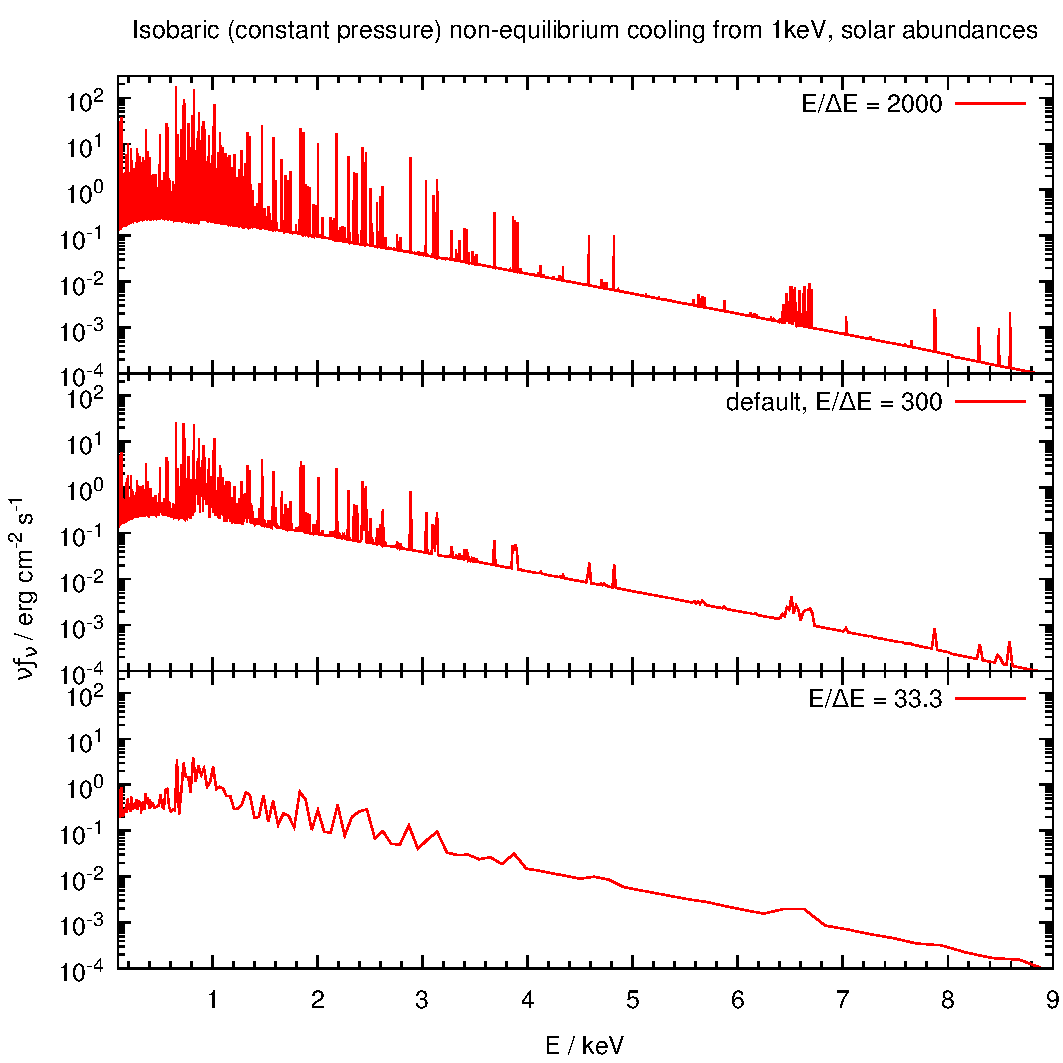
\includegraphics[scale=0.9]{cooling-flow-spectrum-hazy1}
	\caption[Cooling flow]
	{	\label{fig:coolingFlow}
		The X-ray spectrum of a unit-volume parcel of gas cooling under conditions
		of constant pressure (isobarically) from X-ray temperatures (1~keV), computed
		at three resolving powers.
		In the top panel, the resolving power is comparable the proposed {\it Athena}
		resolving power around 6~keV.
		In the bottom panel, the resolving power is comparable to the {\it Chandra}
		non-dispersive resolving power around 1~keV.
		In the middle panel, the resolving power is at the code default.
		This functionality is described in \citet{Chatzikos2015}.
	}
\end{figure}


\begin{shaded}
\section{\protect\experimental Time-variable incident radiation field}
\label{sec:TimeVariableRadiationFields}

This follows the time-dependent evolution of a cloud near a variable
continuum or heat source.

Time-dependent calculations are done by setting up an initial geometry
using the usual commands that specify a cloud and
the incident radiation field.
The \cdCommand{time} keyword establishes which energy sources
vary with time.
The keyword can appear on any of the commands that specify the
luminosity of the radiation field and
on the \cdCommand{hextra} command.
The \cdCommand{trace} option will turn on trace printout.

If a \cdCommand{time} command also occurs
then all radiative and heat sources with
the \cdCommand{time} keyword will change with time.
The \cdCommand{time} command sets a time step
and stopping time.
Each iteration is a time step and the number of time
steps is set with the \cdCommand{iterate} command.
The calculation will stop when
either the number of iterations or the stopping time is reached.

\subsection{time command}

The first argument on the \cdCommand{time} command
is the log of the initial time step in seconds.
The calculation starts at time zero and
the first time step will be this long.
Later time steps will
have their size adjusted by the rate of change in conditions in the gas.
The optional second number gives the log of the stopping
time in seconds.
The calculation will stop when either this time or the number of iterations is reached.

The \cdCommand{time} command is followed by a table giving the logs of
the elapsed time (seconds) and the log of a scale factor giving the
brightness of the variable radiation source relative to the value
specified in the luminosity command.  

The variation of luminosity is linearly interpolated between the 
points specified: the first point gives the initial scale factor.
The code will not extrapolate to times
beyond the end of the table, but for one exception.  If the keyword \cdCommand{cycle}
appears on any line specifying an elapsed time, the code will treat that time as a
period and repeat all previous time steps with that period (the specified period
must be greater than all previously-specified elapsed times).
It will stop if it needs to look up times
beyond the last tabulated value.
The following is a simple example:
\begin{verbatim}
# set the continuum and a variable flux of H-ionizing photons
blackbody T=4e4 K
phi(H) 13.5 time
# set a limit of 50 time steps.  The calculations will actually
# stop when we reach total age
iterate 50 times
# the time command sets a time step of 1e7 s and a stop time of 1e8 s.
# This requires ten time steps.  We set 50 iterations above but the
# calculation will actually stop when the age of 1e8 s is reached.
# The time command is followed by a table giving the log of the age and the
# log of the brightness of the energy source relative to its initial value.
# The table ends with the line saying "end of times"
time steps=7 s stop at 8 s
age = 0 scale = 0
age = 7.3 scale = 0
age = 7.35 scale = 5
age = 7.5 scale = 5
age = 7.55 scale = 0
age = 10 scale = 0
end of times
# commands to set hydrogen density, only done one zone
hden 5
stop zone 1
\end{verbatim}

In this example only one radiation field is given and the flux of
hydrogen-ionizing photons varies with time.  A constant time step of $10^7$~s is used.
The \cdCommand{time} command is followed by the series of lines giving the
brightness of the incident radiation field as a function of time.
The series ends with the line
starting with \cdCommand{end}.
Each of the lines in the age---brightness table starts
with \cdCommand{age} but these characters are ignored.
They are only present to improve readability.

\subsection{Time-step size increment}
\begin{verbatim}
# first set the continuum
blackbody T=4e4 K
# this continuum will vary with time
ionization parameter -2 time
# the CMB will be constant
CMB
# do 50 time steps
iterate 50 times
# the time command itself, followed by a table of times & continua
time 7.5
 7     scale= 0
 7.1   scale=-5 recombination
 9.3   scale=-5
 9.301 scale= 0 ionization, factor = 1.1
 20    scale= 0
end of time
\end{verbatim}
In this example the incident radiation field is a blackbody
with its intensity set by an ionization parameter.
The code does fifty iterations with a time step of
$10^{7.5} \s$ since this is specified on the initial \cdCommand{time} command line.
In the
table the blackbody is left at its initial brightness
for the first $10^7 \s$ then
lowered to $10^{-5}$ of the initial value
for a total of $10^{9.3} \s$ when it is
raised back to the initial value.

As given above, the time steps always have the same size, the size given
on the initial \cdCommand{time} command.
It is also possible to specify the size
of the time step for each elapsed time that appears in the
table that gives the continuum brightness.
If all of the optional time-step sizes are
specified then they are used in place of the time step given on the
\cdCommand{time} command.
The time step sizes are multiplicatively increased by the time-step
scale factor.
It is also possible to give a time-step scale factor saying
how to increase the time step.

If any are missing then the time step on the command is used and is kept
constant.
The table ends with a line saying \cdCommand{end}.
If the optional end
time is not specified on the \cdCommand{time} command
then the calculation will continue
until the specified number of iterations has been performed.

\subsection{Keywords on individual time-step entries}

Most of the letters on the lines giving the times and scale factors are
totally ignored.  They are there to make the table easier to read.  There
are keywords which indicate that a particular time step marks the start
of a special case, such as the recombination of a highly ionized gas or
the propagation of an ionization front into neutral gas.

The keyword \cdCommand{recombination} indicates that
this time step is the first
where the continuum source will be dramatically fainter.
Certain heuristics
are used to follow the recombination and cooling of the gas.

The recombination heuristics are not complete
and the ionization heuristics do not exist..

\subsection{Varying individual continua}

The keyword \cdCommand{time} is used to specify which continua
will be scaled with
time and can appear on any of the luminosity / intensity commands given
in Chapter \ref{sec:IncidentRadiationFieldLuminosity}.
This makes it possible to vary only some of the continua
while others are left constant.
For instance, a constant CMB and a variable
star can be treated.
At least one of the luminosity commands must have
a \cdCommand{time} keyword for time-dependent calculations to be done.

The \cdCommand{hextra} command includes the \cdCommand{time} keyword.
The variable scale factor will apply to the extra heating in this case.

\subsection{Controlling the number of time steps}

Each iteration is a time stop.
The \cdCommand{iterate to convergence} command has a special
meaning in time-dependent calculations.
In this case it tells the code to keep performing iterations,
stepping through time, until one of the special criteria set with a
\cdCommand{stop time} command is satisfied.
The following \cdCommand{stop time} commands are implemented.

\subsubsection{Stop temperature time [exceeds]}

The \cdCommand{stop temperature} command
is described on
page \pageref{sec:CommandStopTemperature}.
It has two forms.  Usually it specifies the lowest temperature
to allow in a calculation.
If the keyword \cdCommand{exceeds} appears then it
specifies the highest temperature to permit.

The \cdCommand{time} keyword tells the code to stop time
when the highest or lowest temperature occurring anywhere
in the computed structure is above or below the limits set
with this command.

\subsection{Other commands}

The \cdCommand{coronal} command has the \cdCommand{time init} option.
This will include thermal collisional ionization for the
initial evaluations of the simulation.
The kinetic temperature will be
free when the time-dependent calculation starts.
\end{shaded}

\section{Wind velocity=300 km/sec [mass =1.4 Msun, disk, ballistic, static]}
\label{sec:CommandWind}

The geometry will be a wind.  The first number is the initial velocity
in \kmps.  The second optional number is the central mass in solar
mass units.  Both are linear quantities.  The previous form of this
command without a \cdCommand{velocity} keyword is now
deprecated.

The equations of motion are solved including the inward pull of gravity.
The gravitational acceleration in the default non-rotating case is
evaluated as
\begin{equation}
g =  - \frac{{GM}}{{r^2 }}\;
 [\cmpss].
\end{equation}
The mass of the central object is given in solar masses
on the command line but is evaluated in gm within the code.
If the mass is not specified then zero is assumed.
If the mass is specified and the keyword \cdCommand{disk} also appears
then the geometry is assumed to be a rotating disk.
In this case the inward
gravitational acceleration~is
\begin{equation}
g =  - \frac{{GM}}{{r^2 }}\left( {1 - \frac{{r_{\mathrm{o}} }}{r}} \right)
\quad [\cmpss]
\end{equation}
where $r_o$ is the inner radius.

The line widths and escape probabilities are evaluated in the Sobolev
or Large Velocity Gradient (LVG) approximation.
The effective line optical depth is given~by
\begin{equation}
\tau_{l,u}(R)=\alpha_{l,u}\min (r,\Delta
r)\left(n_l-n_u\frac{g_l}{g_u}\right)\left(\frac{u_{th}}{\max
(u_{th},u_{\mathrm{exp}})}\right)\quad
  [\mathrm{Napier}]% (68)
\end{equation}
where $u_{th}$ and $u_{\mathrm{exp}}$ are the thermal and expansion
velocities respectively
and the radius used is the smaller of the depth or the radius.
This is
necessary to keep the effective column density from becoming larger than
the total cloud column density when the radius is large and the expansion
velocity is small.

\subsection{Ballistic solutions}

A \cdCommand{ballistic} flag (or \emph{positive velocity} in the case
with no \cdCommand{velocity} keyword) indicates the hypersonic
wind solution that has been a part of the code since its beginnings.
(Note that the negative velocity case has however not yet been tested
thoroughly.)  The equations of motion of the gas are solved, not
including forces due to material pressure gradients.  Acceleration due
to line and continuous opacity of the gas and deceleration due to the
gravity of the central object are included.  The calculation will stop
if the gas comes to rest or if any of the other stopping criteria is
met.  The initial velocity must be above the sonic point.  Further
details are presented in a section in Part~2.

The first parameter is the expansion velocity $u_{\mathrm{o}}$ at the
illuminated face of the cloud.  The approximations used are only
correct if the flow speed remains well above the sound speed
throughout the structure.  The initial velocity is entered in \kmps.
The density at the illuminated face of the cloud is entered with the
\cdCommand{hden} command and the density is varied across the model to
conserve mass flux (i.e., the product $\rho ( r )r^2 u( r )$ is kept
constant).  Because of this a filling factor would not make physical
sense and should not be used (although it can be).  The optional
second parameter is the mass of the central star in solar units; its
default value is one solar mass.

\begin{shaded}
\experimental Without a \cdCommand{ballistic} flag (or A
\emph{negative velocity} in the case with no \cdCommand{velocity}
keyword) the code simulates the flow including corrections due
to pressure gradients in the flow, appropriate to a weak-D or
D-critical \hii\ region (\citealp{Henney2005}).  (Note that the
positive velocity case has however not yet been tested thoroughly.)
This physics is currently under development in collaboration with Will
Henney and Robin Williams.  The central object mass is set to zero.

\subsection{\experimental wind advection, velocity=-5 km/s}

The \cdCommand{advection} keyword says to include the effects of
advection on the
thermal and ionization equations.
Currently advection is only treated in
the case where the velocity is negative, corresponding to a flow off a
molecular cloud towards the source of ionizing radiation.
The argument
is the initial gas flow speed in \kmps.
This physics is being developed
in collaboration with Robin Williams and Will Henney and
is not yet mature.

The advection case has the following options.
In all cases the numerical
parameter follows the keyword.
There can be many parameters on one command line.

\begin{description}
\item[velocity-] The number following this keyword is the velocity in
km~s$^{-1}$.
The following would specify a simple R-type front

\item[center, index-] A varying mass flux with depth into the grid is specified
by a law $\rho u = \Phi _o (r-c)^i $.
This gives the variation in flux
with distance $r$ into the grid as
a function of value $c$ given by the \cdCommand{center} parameter
and the value $i$ given
by the \cdCommand{index} parameter.
For example,
\begin{verbatim}
wind advection velocity -20 center 1e16 index -2
\end{verbatim}
would correspond to a wind diverging spherically
from a point 10$^{16}$ cm into
the grid with a velocity of 20 \kmps\ at the illuminated face.
By default the mass flux is constant ($i = 0$).
If these are not specified then zero is assumed.

\item[dfdr-] This specifies the mass flux gradient, $\Phi ' = d\;\rho u/dr$
[g cm$^{-3}$ s$^{-1}$],
as an alternative to specifying the velocity.
This is
useful in the case in which the flow reaches stagnation at the surface of
the model, in which case the velocity itself does not fully constrain the
physical parameters.

\item[wind advection dfdr-] 20.90 index 2
\end{description}

The \cdCommand{set dynamics} command described below
controls many details of the dynamics.
The \cdCommand{set dynamics pressure mode} command tells the code
whether it should search for globally subsonic or supersonic solution.
If this is not specified the code will compare the ram and gas pressure
at the illuminated face to try to determine whether a super- or sub-sonic
solution is appropriate.

\cdTerm{Convergence-} the level of convergence can be estimated by
comparing the discretization error and convergence error as
a function of iteration, as
shown in Figure 4 of \citet{Henney2005}.
\end{shaded}

\subsection{Wind 5 km/s no continuum }

The \cdCommand{no continuum} keyword tells the code not to include continuous
absorption in the calculation of the radiative acceleration.

The \cdCommand{no induced processes} command will turn off line
radiative acceleration.  It has other physical consequences since
all fluorescent excitation processes are turned off.

\begin{shaded}
\section{\experimental Miscellaneous dynamics commands}

\subsection{Constant pressure time}

This allows the pressure to vary with time.
See Section \ref{sec:ConstantPressureTimescale}
\cdSectionTitle{\refname{sec:ConstantPressureTimescale}}
for more details.

\subsection{Set dynamics [options]}

This changes some aspects of the dynamics solutions when advective winds
are used.
\begin{description}
\item[set dynamics advection  length [fraction]]  This sets the look-back
distance used for the advection terms in the initial iterations of the
solutions.
Its optimum value is determined by a compromise between speed
of convergence (which is improved for large lengths)
and accuracy (which
is improved for small lengths).
The code automatically cuts the look-back
distance when good convergence is obtained so a reasonably large
value can be assumed initially.

If the keyword \cdCommand{fraction} occurs then the
number on the line will be the
fraction of the total depth of the model.
It is the log of the fraction
if it is negative.
If fraction does not occur then the number is the log
of the scale length in~cm.

\item[set dynamics antishock depth 16] would put an
anti-shock at a depth of 10$^{16}$~cm.

\item[set dynamics antishock Mach 1.01] would put in
an anti-shock when the
mach number fell below 1.01.

\item[set dynamics population equilibrium]
This uses the equilibrium solution rather than the non-equilibrium
solution that is done in a dynamical or time-dependent model.

\item[set dynamics pressure mode] This changes some aspects
of how the pressure
solver deals with the sonic point.  The options are: \cdCommand{original},
\cdCommand{subsonic},
\cdCommand{supersonic}, and \cdCommand{strongd}.
The default chooses subsonic or supersonic based
on a comparison of the ram pressure and gas pressure at the face.
\cdCommand{Original}
mode uses similar criteria to choose in each zone but is liable to
oscillation.  \cdCommand{Subsonic} and \cdCommand{supersonic} will force a globally subsonic or
supersonic solution.
\cdCommand{Original} and \cdCommand{strongd} can pass through a
sonic point.
\cdCommand{Strongd} does this by following the supersonic branch
until there is no valid
pressure solution, then following the minimum of the pressure-density
relation until it can leave along the subsonic branch.
By varying the face
conditions, the depth of the internal region of
unphysical solution values
can be minimized, to converge on a physical strong-D type solution.

\item[set dynamics shock depth.]  The argument is
the log of the shock depth in cm.

\item[set dynamics relax 4.]  
This gives the number of static iterations
to be performed before
dynamical or time-dependent behavior begins.
The initial iterations are
done to establish the equilibrium geometry, optical depth scale, and
other properties.
The default is to do 3 iterations to relax the solution.
\end{description}
\end{shaded}

\section{Useful output options}

\subsection{Print cumulative lines}

This gives the time-integrated energy in the emission lines
reported in the main printout.
See page \pageref{sec:CommandPrintLineCumulative} for a description
of this command.

\subsection{Save commands, general comments}

\cdCommand{Save} commands count every time step
counting as an iteration.
If you specify the \cdCommand{last} option you will only
obtain save output for the last time step.

\subsection{Save cumulative continuum}

This gives the time-integrated cumulative energy in the
spectrum reported in the \cdCommand{Save continuum} command.
See page \pageref{sec:CommandSaveCumulativeContinuum} for a
description of this command.

\subsection{Save time dependent}

This gives some information about each time step.
See page \pageref{sec:SaveTimeDependent} for more
information.

\subsection{Set cumulative}

Time-integrated calculations for emission lines and continuua are permitted.
This command controls the weight each timestep receives in the integration,
and it is fully described in Section \ref{sec:SetCumulativeCommand}.

\subsection{Set save hash options}

The \cdCommand{set save hash} command
(page \pageref{sec:CommandSetSaveHash})
has a \cdCommand{time} option to
include the time on every time step in save output. 
